% Created 2015-06-01 Mon 16:14
\documentclass[11pt]{article}
\usepackage[utf8]{inputenc}
\usepackage[T1]{fontenc}
\usepackage{fixltx2e}
\usepackage{graphicx}
\usepackage{longtable}
\usepackage{float}
\usepackage{wrapfig}
\usepackage{rotating}
\usepackage[normalem]{ulem}
\usepackage{amsmath}
\usepackage{textcomp}
\usepackage{marvosym}
\usepackage{wasysym}
\usepackage{amssymb}
\usepackage{capt-of}
\usepackage{hyperref}
\tolerance=1000
\usepackage{minted}
\usepackage{color}
\usepackage{listings}
\usepackage{grffile}
\definecolor{mintedbackground}{rgb}{0.95,0.95,0.95}
\usepackage[inline]{enumitem}
\usepackage{xcolor}
\hypersetup{
colorlinks,
linkcolor={red!50!black},
citecolor={blue!50!black},
urlcolor={blue!80!black}
}
\usepackage{setspace}%% The linestretch
\singlespacing
\usepackage[format=hang,indention=0cm,singlelinecheck=true,justification=raggedright,labelfont={normalsize,bf},textfont={normalsize}]{caption} %
\usepackage{vmargin}
\setpapersize{A4}
\setmarginsrb{2.5cm}{1cm}% links, oben
{2.5cm}{2cm}% rechts, unten
{12pt}{30pt}% Kopf: Höhe, Abstand
{12pt}{30pt}% Fuß: Höhe, AB
\usepackage{upquote}
%  use straight quotes when printing a command in minted
\AtBeginDocument{%
\def\PYZsq{\textquotesingle}%
}
\setlength{\parindent}{0pt}
\setlength{\parskip}{\baselineskip}
\definecolor{mintedbackground}{rgb}{0.95,0.95,0.95}
\author{Alexander Jueterbock, Martin Jakt\thanks{University of Nordland, Norway}}
\date{\textbf{PhD course: High throughput sequencing of non-model organisms}}
\title{\textbf{Trimming and quality control} (2015-06-03)}
\hypersetup{
 pdfkeywords={},
  pdfsubject={},
  pdfcreator={Emacs 24.3.1 (Org mode 8.3beta)}}
\begin{document}

\maketitle
\tableofcontents







After a general introduction to the UNIX command line, it is time for
you to analyze your own fastq files. The first important step for any
kind of sequencing data is to get rid of adapter contamination and 
bad quality reads. In this tutorial we will use the programs \href{http://www.bioinformatics.babraham.ac.uk/projects/fastqc/}{FastQC}
and \href{http://www.bioinformatics.babraham.ac.uk/projects/trim_galore/}{TrimGalore!} to check the quality of the sequenced libraries before
and after trimming. We will also learn few more UNIX commands that
extract important information from fastq files and that allow you to
turn off your computer while the analysis continues to run on the
remote server.


\textbf{IMPORTANT NOTE} Before you get started: to compare characteristics of
your libraries, please keep record of the resulting numbers, like the
number of raw reads, reads after quality control, number of mapped
reads etc. This helps to identify peculiarities/outliers in your
libraries which may either be due to biological peculiarities of your
species or unknown technical issues.


Log on (with \texttt{ssh}) to the remote computer with the \texttt{-X} option to be
able to use graphical interfaces.

\section{Overview of sequence lengths}
\label{sec-1}
Next Generation Sequencing data is generally stored in fastq
files. Most of the time the data are compressed, either in .zip or in
.gz format.

If your file is zip-compressed, you can use the following command to unzip it:

\begin{minted}[fontsize=\scriptsize,bgcolor=lightgray,linenos]{sh}
unzip FILE.fastq.zip
\end{minted}

If your file iz gz-compressed, use the following command instead:

\begin{minted}[fontsize=\scriptsize,bgcolor=lightgray,linenos]{sh}
gunzip FILE.fastq.gz
\end{minted}


To get a quick impression of the minimum and maximum read lengths in
your fastq file, you can use the following commands (replace
\texttt{FILE.fastq} with your own filename):

\begin{minted}[fontsize=\scriptsize,bgcolor=lightgray,linenos]{sh}
awk '{if(NR%4==2) print length($0)}' FILE.fastq| sort -n | head -n1
awk '{if(NR%4==2) print length($0)}' FILE.fastq| sort -n | tail -n1
\end{minted}

It reads like this: measure the length of every second line in every
group of 4 lines (the sequence line in a fastq file), \texttt{sort} it
(numerically with \texttt{-n}) and print out either the first (smallest)
value with \texttt{head} or the last (biggest) value with \texttt{tail}. \texttt{NR}
represents the current line number and the \texttt{\%} sign is the modulus
operator, which divides the line number by 4 (\texttt{NR\%4}) and returns only
the remainder. This extracts all the sequences, which are on line
2,6,10,14\ldots{}


The following command allows you to count the sequence lengths:

\begin{minted}[fontsize=\scriptsize,bgcolor=lightgray,linenos]{sh}
awk '{if(NR%4==2) print length($0)}' FILE.fastq | sort -n | uniq -c > read_length.txt
\end{minted}

The lines that follow makes use of the program R. If you copy and
paste the code into the command line, you will get an overview graphic
of the sequence length distribution 

\begin{minted}[fontsize=\scriptsize,bgcolor=lightgray,linenos]{sh}
cat >> Rplot.r << 'EOF'
reads<-read.csv(file="read_length.txt", sep="", header=FALSE)

png(filename = "SequenceLengthDistribution.png",
         width = 480, height = 480, units = "px", pointsize = 12,
          bg = "white")
plot(reads$V2,reads$V1,type="l",xlab="read length",ylab="occurences",col="blue")
dev.off()

EOF


R CMD BATCH Rplot.r
\end{minted}

You can open the created figure with the GNOME image viewer using the
following command:

\begin{minted}[fontsize=\scriptsize,bgcolor=lightgray,linenos]{sh}
eog SequenceLengthDistribution.png
\end{minted}


\begin{figure}[htb]
\centering
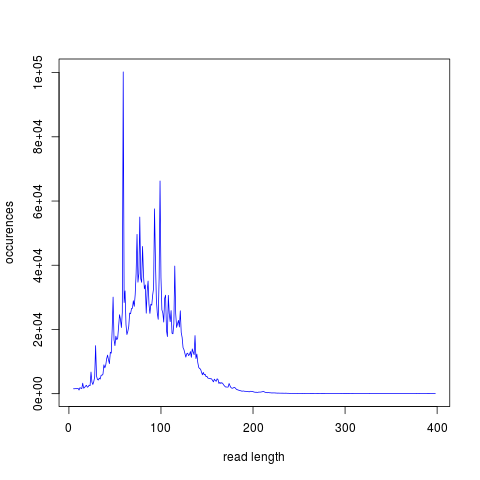
\includegraphics[width=10cm]{SequenceLengthDistribution.png}
\caption{Example graphic of the length distribution in a fastq file}
\end{figure}




\section{Quality control}
\label{sec-2}
To inspect the quality of the sequencing data, we use
\href{http://www.bioinformatics.babraham.ac.uk/projects/fastqc/}{FastQC}. In
the installation and setup instructions of the program
(\href{http://www.bioinformatics.babraham.ac.uk/projects/fastqc/INSTALL.txt}{link}),
you will find that FastQC can run in an interactive mode or in a
command line mode. This tutorial uses the command-line version but
feel free to play around yourself with the interactive version of
FastQC.

FastQC knows a number of standard adapter sequences used for HTS; however,
it is not aware of the sequences used by the IonTorrent platform. To
inform FastQC of the adapter sequences we have used we call FastQc with the
\texttt{-a}, or \texttt{-{}-adapters} option to specify a file containing the adapter
sequences we have used.

So, to run FastQC on your file, simply type (where adapters.txt is a file
containing the adapter sequences in a suitable format):

\begin{minted}[fontsize=\scriptsize,bgcolor=lightgray,linenos]{sh}
fastqc -a adapters.txt FILE.fastq
\end{minted}

The output will be saved in a folder that has the name of your fastq
file and ends with fastqc, like \texttt{FILE\_fastqc}. Use the \texttt{cd} command to
move into the folder and open the produced \texttt{fastqc\_report.html} either
with \texttt{firefox} or \texttt{chromium-browser} (one of the two should work). 

\begin{minted}[fontsize=\scriptsize,bgcolor=lightgray,linenos]{sh}
firefox fastqc_report.html
chromium-browser fastqc_report.html
\end{minted}

Get familiar with the output. Does the sequence length-distribution
meet your expectations (400bp library)? You can find guidance on how to 
interpret the output of each module \href{http://www.bioinformatics.babraham.ac.uk/projects/fastqc/Help/3\%20Analysis\%20Modules/}{here}.

\section{Trimming low quality reads and adapters}
\label{sec-3}


\href{http://www.bioinformatics.babraham.ac.uk/projects/trim_galore/}{TrimGalore!} is a wrapper script to automate quality and adapter
trimming as well as quality control (\href{http://www.bioinformatics.babraham.ac.uk/projects/trim_galore/trim_galore_User_Guide_v0.3.7.pdf}{User Guide}).

When the program is installed, it can be used with 

\begin{minted}[fontsize=\scriptsize,bgcolor=lightgray,linenos]{sh}
trim_galore [options] <filename(s)>
\end{minted}

You can get an overview of the options with the \texttt{-{}-help} option:

\begin{minted}[fontsize=\scriptsize,bgcolor=lightgray,linenos]{sh}
trim_galore --help
\end{minted}

With the default settings, TrimGalore! trims low-quality ends with a
Phred quality score threshold of 20 (can be changed with \texttt{-q}) and
discards reads that become shorter than 20 bp (can be changed with
\texttt{-{}-length}).

The Ion-P1- and Ion-A-adapters are supposed to be automatically
trimmed off on the Ion Server. So, the fastq files with the raw reads
should not contain these adapters anymore. Nevertheless, try to trim them
off anyway in order to check if there are still adapters left in your
library - they can have negative effects on further analyses.

TrimGalore! uses the program \href{https://code.google.com/p/cutadapt/}{Cutadapt} to find and remove adapters from
the 3' end of the reads (see Fig. \ref{fig:adapters}). The program Cutadapt
itself gives you more options for adapter trimming and allows you to
remove adapters from the 5'-end of the sequence (see
\url{http://cutadapt.readthedocs.org/en/latest/guide.html})

\begin{figure}[htb]
\centering
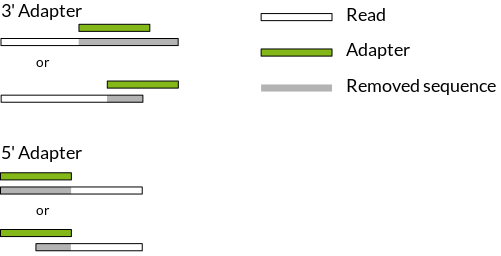
\includegraphics[width=14cm]{adapters.png}
\caption{\label{fig:adapters}3'- and 5'-adapter trimming (\href{http://cutadapt.readthedocs.org/en/latest/guide.html}{source})}
\end{figure}


The adapters used for Ion Torrent sequencing are shown in
Fig. \ref{fig:ionadapters} and their orientation in the libraries is shown
in Fig. \ref{fig:adapterorientations}.

\begin{figure}[htb]
\centering
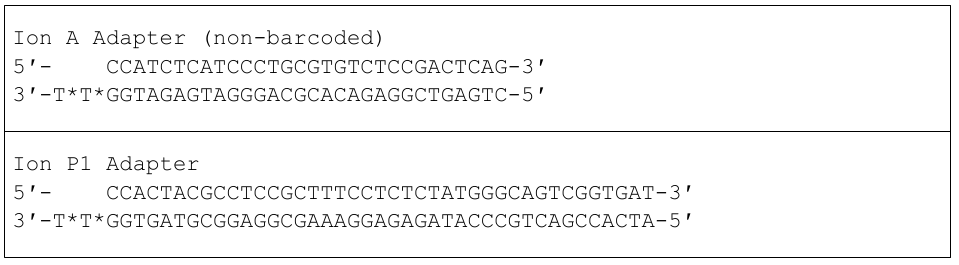
\includegraphics[width=14cm]{IonAdapters.png}
\caption{\label{fig:ionadapters}Non-barcoded Ion-A and -P1 adapter sequences. In each sequence, a "*" indicates a phosphorothioate bond, for protection from nucleases and to preserve the directionality of adapter ligation}
\end{figure}

\begin{figure}[htb]
\centering
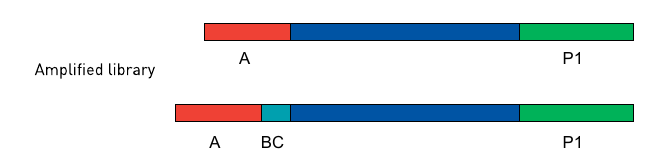
\includegraphics[width=14cm]{IonLibraryWithAdapters.png}
\caption{\label{fig:adapterorientations}Ion adapters in the amplified library. BC is an optional barcode sequence.}
\end{figure}.

To trim off the A-adapter, use TrimGalore! with the command:

\begin{minted}[fontsize=\scriptsize,bgcolor=lightgray,linenos]{sh}
trim_galore \
-a CCATCTCATCCCTGCGTGTCTCCGACTCAG \
--stringency 3 \
FILE.fastq
\end{minted}

The \texttt{\textbackslash{}} sign just means that the command continues on the next
line. You could type the entire command on a single line.


The option \texttt{-{}-stringency 3} means that a >3bp overlap with the adapter
sequence will be trimmed off the 3' end. The program writes a file
that ends with \texttt{trimming\_report.txt}, which reports the number of
reads that have been trimmed and/or removed.

The output file has the ending \texttt{trimmed.fq}. Use this file as
input to TrimGalore! to trim off the P1-adapter:

\begin{minted}[fontsize=\scriptsize,bgcolor=lightgray,linenos]{sh}
trim_galore \
-a CCACTACGCCTCCGCTTTCCTCTCTATGGGCAGTCGGTGAT \
--stringency 3 \
--fastqc FILE_trimmed.fq
\end{minted}

The \texttt{-{}-fastqc} option will automatically run FastQC in the default
mode. Compare the FastQC outputs before and after trimming.


\clearpage

\section{Fraction of duplicate reads}
\label{sec-4}
Duplicate reads (identical reads present more than once in the
library) can skew genotype estimates and thus should be identified and
removed before SNP calling. Duplicates can result from primer or PCR
bias towards these reads and poor libraries can have levels of
duplicates >50\%.

At this step, we will calculate the fraction of duplicates but we will
remove them only after \emph{de novo} genome assembly and read mapping.
The approach is based on the \href{http://sfg.stanford.edu/SFG.pdf}{Simple fool's guide to population
genomics via RNAseq} and makes use of \texttt{fastx\_collapser} from the
\href{http://hannonlab.cshl.edu/fastx_toolkit/}{FASTX-Toolkit} and a python script (\texttt{fastqduplicatecounter.py}).

First, use \texttt{fastx\_collapser} to combine and count all identical reads.

\begin{minted}[fontsize=\scriptsize,bgcolor=lightgray,linenos]{sh}
fastx_collapser -Q 33 -v -i INPUTFILE.fq -o OUTPUTFILE.txt
\end{minted}

The \texttt{INPUTFILE} is your trimmed fastq file. \texttt{-Q 33} specifies that
quality scores are Phred33 encoded.  The \texttt{OUTPUTFILE} is used in the
next step with the python script 'fastqduplicatecounter.py'.

\begin{minted}[fontsize=\scriptsize,bgcolor=lightgray,linenos]{sh}
fastqduplicatecounter.py OUTPUTFILE.txt OUTPUTFILE_header.txt > OUTPUTFILE_duplicatecount.txt
\end{minted}

This script calculates the fractions of duplicate and singleton
reads. Open the outputfile with \texttt{less OUTPUTFILE\_duplicatecount.txt}
and check the percentage of duplicate reads.
\section{BONUS Running programs in the background with \texttt{nohup}}
\label{sec-5}
What if your data analysis on a remote server takes several hours,
days, or even weeks, to finish? No worries, you don't need to be
connected to the remote server while the data are being
analysed. Here, you will learn the tools that allow you to start
an analysis, disconnect from the server, and then look at the progress
or the results at a later time point.

The \texttt{nohup} tool allows you to run a process in the background; which
means that, while the analysis is running, you can do other tasks in
parallel or log off from the remote server.

Imagine the \texttt{nohup} tool as a bracket which encloses the command that
you want to run in the background:

\begin{minted}[fontsize=\scriptsize,bgcolor=lightgray,linenos]{sh}
nohup ... &
\end{minted}

Always, \texttt{nohup} precedes and \texttt{\&} follows the command that you want to
run in the background (here shown as \texttt{...}). Let's say you want to run
the command \texttt{ls -lhcrt} (which lists all files and subdirectories in
your current directory) in the background.

\begin{minted}[fontsize=\scriptsize,bgcolor=lightgray,linenos]{sh}
nohup ls -lhcrt &
\end{minted}

When you hit ENTER, the terminal prints out some information:

\begin{minted}[fontsize=\scriptsize,bgcolor=lightgray,linenos]{sh}
[1] 21118
nohup: ignoring input and appending output to 'nohup.out'
\end{minted}

The number \texttt{21118} (which will differ in your case) in the first line
is the process-ID of your background-process. The second line informs you that
all 'results', that would be normally printed in the terminal window,
are now redirected to the file \texttt{nohup.out}. 

\subsection{Using the process-ID}
\label{sec-5-1}
If you have started a process that takes several hours
to finish, then you can use the process-ID to see if the process is
still running. For this, you can use the \texttt{ps} command with the \texttt{-p}
option, which reports the status of a process with a certain process
ID. To see the status of the process I have started above, I would
use:

\begin{minted}[fontsize=\scriptsize,bgcolor=lightgray,linenos]{sh}
ps -p 21118
\end{minted}

The output is

\begin{minted}[fontsize=\scriptsize,bgcolor=lightgray,linenos]{sh}
PID TTY          TIME CMD
\end{minted}

Since this is only the header line of the process specifications, the
process must have finished. 
Here:
\begin{itemize}
\item \texttt{PID} indicates the process-ID
\item \texttt{TTY} indicates the controlling terminal
\item \texttt{TIME} shows the time that the process is running already
\item \texttt{CMD} shows the command name
\end{itemize}

If the process would still run, you would
get a line similar to:

\begin{minted}[fontsize=\scriptsize,bgcolor=lightgray,linenos]{sh}
PID  TTY          TIME CMD
21118 ?        00:00:04 ls
\end{minted}

The \texttt{top} tool provides an ongoing look at processor activity in real
time, similar to Figure \ref{fig:top}.


\begin{figure}[htb]
\centering
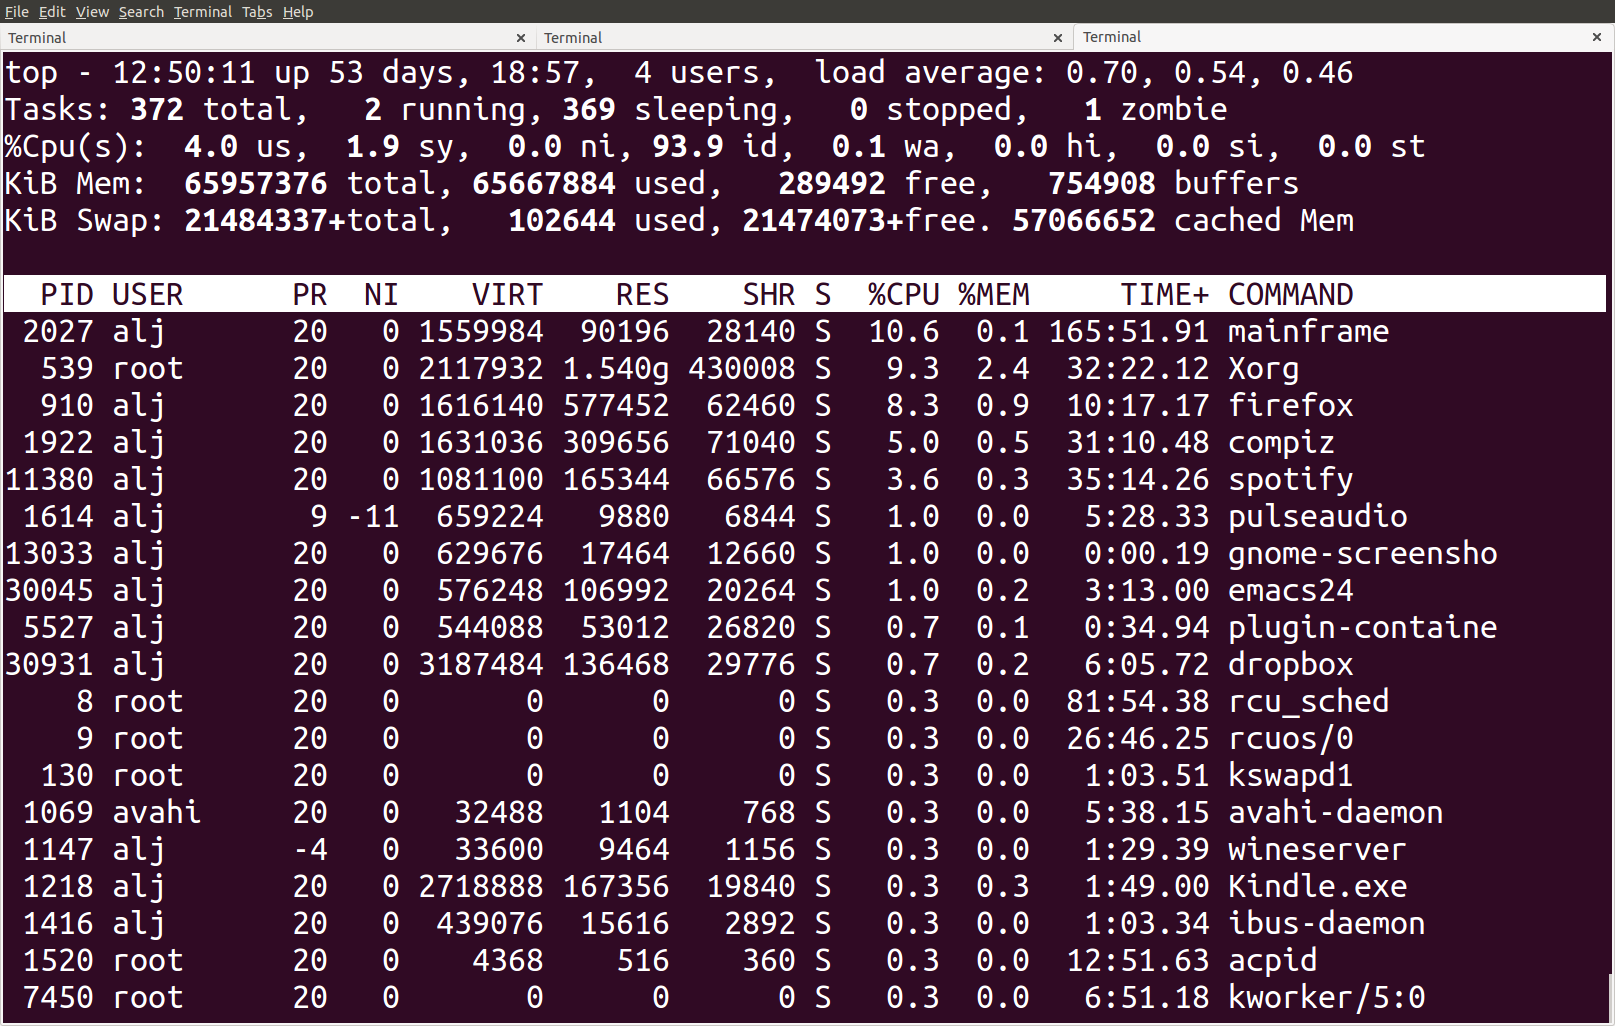
\includegraphics[width=10cm]{top.png}
\caption{\label{fig:top}Screenshot of the \texttt{top} tool output}
\end{figure}

At the top of the screen, it lists processes ordered by their CPU usage
system (with the most intensive on top). Besides other information, it shows which user is running
which process, as well as the process-ID. You can quit the program by
hitting \texttt{q}.

The process-ID also allows you to cancel the process before it
finishes. Cancelling processes comes in handy when you figure out
that you started them with the wrong parameters or input files and you want
to re-start with different settings. The \texttt{kill} command allows you
to cancel a specific process.

\begin{minted}[fontsize=\scriptsize,bgcolor=lightgray,linenos]{sh}
kill 21118
\end{minted}

This would cancel the process that we started before in the
background. If you can't remember the process-ID but want to cancel
all \texttt{ls} processes, then you could use the \texttt{pkill} command in the
following way:

\begin{minted}[fontsize=\scriptsize,bgcolor=lightgray,linenos]{sh}
pkill ls
\end{minted}

Compared to the \texttt{kill} command, the \texttt{pkill} command allows you to
specify the command-name instead of the process-ID of the running
process that you want to cancel.

If you don't have a record of the PID you can find out the id of processes being run by a specific user
by combining \texttt{ps} and \texttt{grep}:

\begin{minted}[fontsize=\scriptsize,bgcolor=lightgray,linenos]{sh}
ps aux | grep user_name
\end{minted}

where \texttt{user\_name} is your own user name. That will list all processes started by
you (well using your id in any case). The \texttt{aux} option specifies all processes and
the manner in which these are printed out. If you read the man file (\texttt{man ps}) you
will see that there are ways in which you can get ps to only list processes started
by the current user (\texttt{ps -eu}) in a similar manner and that \texttt{ps aux} is BSD syntax.
So \texttt{grep} isn't really needed here, but I tend to like the way this formats the output.

\subsection{Redirecting output}
\label{sec-5-2}
By default, the \texttt{nohup} command redirects all information from the
terminal window to the \texttt{nohup.out} file. If the file exists already,
it will not be overwritten. All new information will be appended to
the end of the file. With the \texttt{>} operator, you can redirect the
output to a different file. For example, to redirect the output of the
\texttt{ls} command to the file \texttt{Directory-Listing.txt}, you can use the
command

\begin{minted}[fontsize=\scriptsize,bgcolor=lightgray,linenos]{sh}
nohup ls -lhcrt > Directory-Listing.txt &
\end{minted}

So, the redirection-operator (\texttt{>}) is followed by the name of the
target file and precedes the closing \texttt{\&} operator of the \texttt{nohup}
command. If you want to save the output to a file in a different
directory, just specify the entire file-path that precedes your target
file, like:

\begin{minted}[fontsize=\scriptsize,bgcolor=lightgray,linenos]{sh}
nohup ls -lhcrt > /home/alj/Documents/DirectoryListing.txt &
\end{minted}
Emacs 24.3.1 (Org mode 8.3beta)
\end{document}